\documentclass[12pt,journal,compsoc]{IEEEtran}
\usepackage[utf8]{inputenc}
\usepackage[ngerman]{babel}
%\usepackage{tikz, tikzscale, adjustbox,enumerate, tabularx, multirow, booktabs}
\usepackage{graphicx, tabularx, booktabs, enumerate, multirow}
\usepackage{cite, textcomp}
\usepackage{hyperref}

\usepackage{listings}
\lstset{
  language=C,
  basicstyle=\ttfamily\small,
  keywordstyle=\color{blue}\ttfamily,
  stringstyle=\color{red}\ttfamily,
  commentstyle=\color{green}\ttfamily\normalsize,
  breakatwhitespace=false,
  breaklines=true
}


\makeatletter
{\obeylines\gdef\bt@eol{^^M}}
\newenvironment{breakabletexttt}
  {\ttfamily\hfuzz=0.4em
   \list{}{\leftmargin=2em
           \itemindent=-\leftmargin
           \listparindent=-\leftmargin
           \parsep=0pt}
   \item\relax\obeylines\obeyspaces\expandafter\breakable@texttt\@gobble}
  {\endlist}
\def\breakable@texttt{\futurelet\@let@token\breakable@texttti}
\def\breakable@texttti#1{%
  \ifx\@let@token\end
  \expandafter\end
  \else
    \expandafter\ifx\bt@eol\@let@token
      \par
    \else
      \string#1\hskip1sp
    \fi
    \expandafter\breakable@texttt
  \fi}
\makeatother



\usepackage{tikz, tikzscale} % tiks für Zeichnungen

\usepackage[europeanresistors,europeaninductors,arrowmos]{circuitikz}
\usepackage{amsmath}

%\usepackage[siunitx]{circuitikz}
%\usepackage[ngerman]{varioref}% Definiert variable Referenzierungen
%\usetikzlibrary{dsp,chains}

\providecommand{\PSforPDF}[1]{#1}
\setcounter{secnumdepth}{1}

% NOTE: PDF hyperlink and bookmark features are not required in IEEE
%       papers and their use requires extra complexity and work.
% *** IF USING HYPERREF BE SURE AND CHANGE THE EXAMPLE PDF ***
% *** TITLE/SUBJECT/AUTHOR/KEYWORDS INFO BELOW!!           ***
\newcommand\MYhyperrefoptions{bookmarks=true,bookmarksnumbered=true,
pdfpagemode={UseOutlines},plainpages=false,pdfpagelabels=true,
colorlinks=true,linkcolor={black},citecolor={black},pagecolor={black},
urlcolor={black},

pdftitle={DIY Wordclock},
pdfsubject={Wordclock},
pdfauthor={Christof Pfannenmüller}}




% correct bad hyphenation here
%\hyphenation{op-tical net-works semi-conduc-tor}


\begin{document} %----------------------------------------------------------------------------Beginn des Dokuments
%
% paper title
% can use linebreaks \\ within to get better formatting as desired
\title{DIY Wordclock}

\author{Christof Pfannenmüller}% <-this % stops a space



  % for Computer Society papers, we must declare the abstract and index terms
  % PRIOR to the title within the \IEEEcompsoctitleabstractindextext IEEEtran
  % command as these need to go into the title area created by \maketitle.
%  \IEEEcompsoctitleabstractindextext{%
%  \begin{abstract}
  %\boldmath
  %The abstract goes here.
%  \end{abstract}
  % IEEEtran.cls defaults to using nonbold math in the Abstract.
  % This preserves the distinction between vectors and scalars. However,
  % if the journal you are submitting to favors bold math in the abstract,
  % then you can use LaTeX's standard command \boldmath at the very start
  % of the abstract to achieve this. Many IEEE journals frown on math
  % in the abstract anyway. In particular, the Computer Society does
  % not want either math or citations to appear in the abstract.

  % Note that keywords are not normally used for peerreview papers.
%  \begin{IEEEkeywords}
%  Computer Society, IEEEtran, journal, \LaTeX, paper, template.
%  \end{IEEEkeywords}}


% make the title area
\maketitle


% To allow for easy dual compilation without having to reenter the
% abstract/keywords data, the \IEEEcompsoctitleabstractindextext text will
% not be used in maketitle, but will appear (i.e., to be "transported")
% here as \IEEEdisplaynotcompsoctitleabstractindextext when compsoc mode
% is not selected <OR> if conference mode is selected - because compsoc
% conference papers position the abstract like regular (non-compsoc)
% papers do!
\IEEEdisplaynotcompsoctitleabstractindextext
% \IEEEdisplaynotcompsoctitleabstractindextext has no effect when using
% compsoc under a non-conference mode.


% For peer review papers, you can put extra information on the cover
% page as needed:
% \ifCLASSOPTIONpeerreview
% \begin{center} \bfseries EDICS Category: 3-BBND \end{center}
% \fi
%
% For peerreview papers, this IEEEtran command inserts a page break and
% creates the second title. It will be ignored for other modes.
%\IEEEpeerreviewmaketitle

%----------------------------------------------------------------------------------------------Beginn des  eigentlichen Textes

\section{Einführung}

\IEEEPARstart{W}{ordclocks} sind in der Bastler oder DIY-Szene weit verbreitet und bergen eine gewisse Faszination. Auch wenn es für solche Wordclocks schon eine Vielzahl an Bauanleitungen gibt, kann trotzdem beim Bau einer solchen viel über die Programmierung und die Steuerung durch Mikrocontroller gelernt werden.
Grundsätzlich sind alle Wordclocks sehr ähnlich aufgebaut. Fast immer wird eine Frontplatte mit passend angeordneten  Buchstaben verwendet, die durch eine Matrix an LEDs von hinten erleuchtet ist. Dadurch, dass nur die zur aktuellen Stunde passenden   Wörter leuchten, stechen diese aus den, auf den ersten Blick verwirrend angeordneten, Buchstaben der Frontplatte hervor. Wichtig bei einer Wordclock ist auch, dass jede LED nur den für sie vorgesehen Buchstaben der Frontplatte beleuchtet und nicht zu einem Teil auch die benachbarten Buchstaben. Dies würde den absetzenden Effekt des Hervorscheinens der Buchstaben von den dunkleren minimieren. Dafür wird meist eine sogenannte Zwischenplatte angebracht, die das Licht der LED abschirmt, damit sichergestellt werden kann, das kein Nachbarbuchstabe beleuchtet wird.
Wordclocks wurden bereits in vielen verschiedenen Sprachen erstellt, wobei  grundsätzlich jede Sprache möglich ist. Die einzige Vorgabe ist alle Wörter, die zum \glqq schreiben\grqq der Uhrzeit notwendig sind, auf der Frontplatte anzuordnen. Dabei ist jedoch wichtig, dass die Reihenfolge der Wörter so gewählt wird, das jede mögliche Uhrzeit auch dargestellt werden kann ohne ein Wort doppelt unterbringen zu müssen und trotzdem die Reihenfolge der Wörter dem Sprachgebrauch entspricht. In diesem Zusammenhang ist etwa die Darstellung der Zeit 15:45 interessant, denn je nach Wohnort wird diese in unterschiedlichem Wortlaut verwendet. Vor allem in Sachsen, Thüringen und Franken wird die Bezeichnung \glqq Dreiviertel vier\grqq verwendet, in Norddeutschland dagegen eher \glqq Viertel vor vier\grqq. Solche Feinheiten müssen also berücksichtigt werden, bei \glqq Viertel nach drei\grqq bzw. \glqq Viertel vier\grqq verhält es sich ähnlich.

\begin{figure}
	\centering
	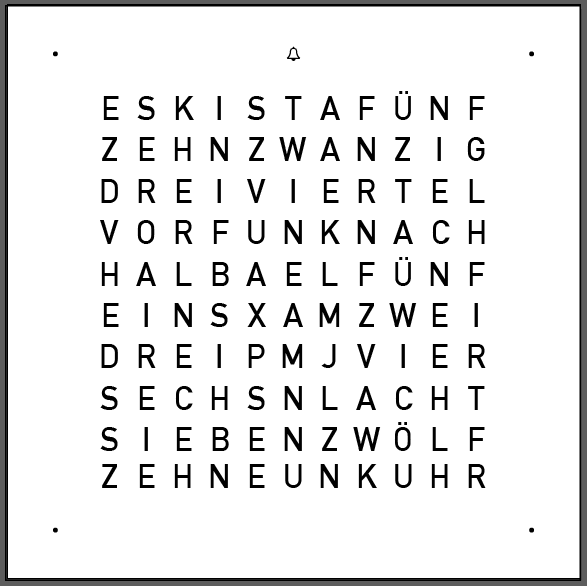
\includegraphics[width=0.45\textwidth]{Bilder/Frontplatte1}
	\caption{Die Frontplatte meiner Wordclock} 
	\label{fig:Frontplatte1}
\end{figure}

\section{Anforderungen}
Diese Wordclock sollte vor allem - im Gegensatz zu den meisten anderen - kleiner ausgelegt und nicht zum Aufhängen an der Wand gedacht sein, sondern als modulare kleine Tischuhr, die bei Einbau einer Alarmfunktion, auch als Wecker dienen kann.
Bei ersten Recherchen fand ich heraus, dass der Hersteller Qlocktwo mittlerweile eine solche Uhr in seinem Sortiment hat. Qlocktwo ist allem Anschein nach der einzige Hersteller von Wordclocks auf dem Europäischen Markt. Da der Hersteller auch Ersatzfrontplatten verkauft, entschied ich mich zuerst eine solche zu kaufen und eine eigene Frontplatte erst zum Schluss zu erstellen, wenn die Wordclock bereits funktionsfähig ist. Dadurch musste ich zwar die geplante Größe der Wordclock um ein paar Zentimeter auf 13,5cm Seitenlänge verkleinern, konnte mich aber erst einmal auf die Elektronik konzentrieren.
Um zunächst einen Überblick zu bekommen sammelte ich alle möglichen Projektideen und mögliche Umsetzungen in einem, mit Latex erstellten, Lasten- und Pflichtenheft. Dabei wurde auch die in Latex integrierte Bibliographieverwaltung verwendet um alle Quellen für Ideen zu archivieren. Zur Versionskontrolle wurde während des Projektes für alle Dateien Github eingesetzt um jeweils den aktuellen Stand zu protokollieren. Das fertige Github-Repository ist unter der \url{https://github.com/pfanchri/Wordclock} zu finden.


\section{Hardware}

\subsection{Eagle}
Für die Platine wird Eagle als PCB-Software zum Entwurf der Platine verwendet, da es kostenlos verwendet werden kann und die Platinenentwicklung im Fablab auf Eagle ausgerichtet ist. Eagle arbeitet nach dem Bibliotheks-Prinzip, das heißt es werden für jedes  Bauteil Daten über die Elektrischen Anschlüsse und über das Package, also über die Verpackung des Bauteils, benötigt. In Eagle können somit  zuerst der Schaltplan, also die elektrischen Verbindungen und Netze, erstellt werden. Diese werden in einem zweiten Schritt auf der Platine angeordnet und die Leiterbahnen geroutet. Hier kann leicht berücksichtigt werden, dass viele elektrische Bauteile in unterschiedlichen Packages zur Verfügung stehen. Die bei der Wordclock verwendeten Bauteile waren zumeist in den mit Eagle ausgelieferten Bibliotheken bereits enthalten. Die Bibliotheksdaten für die LEDs waren zwar nicht in den Standartbibliotheken enthalten, werden dafür aber von Adafruit, einem Händler für diese Bauteile, bereitgestellt. Im Layout wurden zuerst alle LEDs an die durch die Frontplatte vorgegebenen stellen platziert. Anschließend wurden die Taster angeordnet, sodass diese später optisch ansprechend platziert sind. Alle in der fertigen Wordclock nicht mehr sichtbaren Bauteile wurden als letztes platziert und mit Leiterbahnen versehen. Eagle konnte auch eingesetzt werden, um etwa eine Stückliste der verwendeten Teile auszugeben.
\begin{figure}
	\centering
	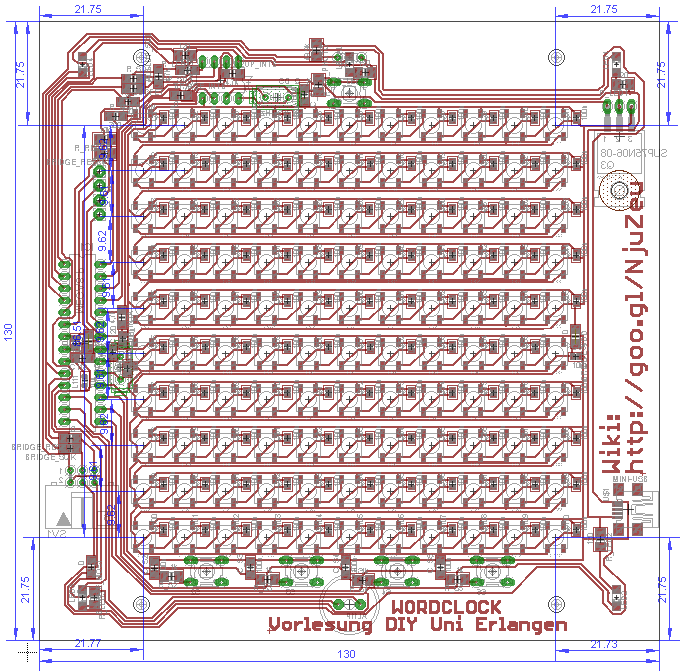
\includegraphics[width=0.45\textwidth]{Bilder/Eagle.png}
	\caption{Das Layout in Eagle} 
	\label{fig:EagleL}
\end{figure}





\subsection{Elektronik}
Das Ziel ist die Platine einlagig aufzubauen. Dies erhöht zwar den Aufwand für das Layout immens, dafür kann aber eine einlagige Platine verwendet werden, die wesentlich einfacher zu entwickeln ist, als eine zweilagige. Auch werden keine Durchkontaktierungen in der Platine benötigt, die im Fablab etwas aufwändiger sind. Da der Platz aber durch die Vorgabe der Frontplatte begrenzt ist, müssen auch kleine Bauteile verwendet werden, die etwas schwieriger zu löten sind.
Versorgt werden soll die Uhr mittels Strom aus einem USB-Ladegerät oder Computer damit kein besonderes Ladegerät notwenig ist. Dies legt die Versorgungsspannung auf 5 Volt fest. Als Stromanschluss wird eine kombinierte Micro-USB-Buchse, die für Stecker des Types A und B geeignet ist, verwendet. Die Uhr kann dadurch mit einem Ladekabel für Handys betrieben werden.
Die Hauptarbeit übernimmt dabei ein Prozessor der  Mega8-Reihe von Atmel, da dieser einfach zu programmieren und leicht verfügbar ist. Genau wird der Atmega168PA-PU verwendet, der den größten programmierbaren Flash seiner Baureihe zur Verfügung stellt. Da ein späterer Einbau einer Batteriepufferung möglich sein soll, verwenden wir hier die Pico-Power Ausführung des AVR, da diese weniger Strom im Schlafmodus verbraucht, was hierbei hilfreich sein kann. Als Baugröße verwende ich hierbei die PDIP  Ausführung . Da bei diesem Gehäuse die Pins nahe beieinander liegen, kann der AVR gut zwischen der LED-Matrix und dem Rand der Platine eingebaut werden. Hierfür wäre eine andere Gehäuseform zu groß. Zum Programmieren des AVR wird eine Standart ISP-Stecker verwendet, da bereits damit zu rechen ist, das die Software mehrfach aufgespielt werden muss, bis diese reibungslos läuft. 
Die LED-Matrix zum Anzeigen der einzelnen Buchstaben der Uhr wird durch 110 WS2812B LEDs aufgebaut. Diese LEDs haben den Vorteil, dass sie eine eigene Datenleitung haben und der Mikrocontroller daher nur einen Pin bereitstellen muss, um alle hundertzehn Buchstaben ansteuern zu können. Dies funktioniert, indem ein, in die LED eingebauter Chip, dieses Datensignal empfängt und über den Data-Out-Pin der LED die folgenden LEDs mit dem Datensignal versorgt. Alle drei Grundfarben können durch den Chip in 255 Stufen bei den LEDs getrennt geregelt werden. Damit kann also mit jedem der 110 Buchstaben das gesamte Farbspekrum von 16777216 verschiedenen Farben dargestellt werden. Dem Datenblatt der WS2812B zufolge sollte bei jeder WS2812B ein Kondensator mit 100nF zwischen Versorgungsspannung und Ground im Layout eingebaut werden. Dies dient dazu die Versorgungsspannung der  LED zu stabilisieren und somit sicherzustellen, das die Ansteuerung richtig funktioniert. Da für die Versorgung des eingebauten Steuerchips der WS2812B auch im ausgeschalteten Zustand Strom benötigt wird, kann die Gesamte Matrix über einen P-Kanal-Mosfet von der Versorgungsspannung getrennt werden.Für die LEDs, welche die einzelnen Minuten und den Alarm anzeigen, werden dagegen \glqq normale\grqq LEDs verwendet, deren Kathode vom Mikrocontroller auf Ground gezogen werden können und damit angeschaltet werden. Um keine ungewollten Aktionen beim Programmieren des Atmega auszulösen werden die LEDs auf die selben Pins des Mikrocontroller gelegt, die auch als Verbindung zum In-System-Programmer dienen. Beim Programmieren des AVR kann es also nun vorkommen, dass  die LEDs aktiviert werden, es kann jedoch kein Schaden an Bauteilen erzeugt werden, obwohl diese Pins doppelt genutzt werden.
Die Uhrzeit soll sowohl im Mikrocontroller selbst als auch in einem externen Realtime-Clock-Baustein gezählt werden können. Der externe Baustein hat hierbei wieder die Vorteile, dass der Atmega168 im Schlafmodus sein kann und somit wenig Strom benötigt wird. Als Clock-Baustein wird hierfür ein DS1337 verwendet, da dieser zwei externe Interrupt Kanäle besitzt und somit den Mikrocontroller durch einen Alarm aus dem Schlafmodus aufwecken kann. Die Real-Time-Clock wird vom AVR über das Two-Wire Protokoll angesteuert werden.
Für das Einstellen der Uhrzeit und das Nutzen anderer Funktionen, wie etwa eines Alarms, wurden fünf Taster verbaut. Alle diese sind mit einem Kondensator entprellt und jeder Taster ist am AVR angeschlossen, sodass ein Tastendruck mit einem Pin-Change-Interrup detektiert werden kann. 
Außerdem wurde ein LDR (Light Dependent Resistor) also ein lichtabhäniger Widerstand eingebaut. Somit kann zu einem späteren Zeitpunkt die Helligkeit der Matrix in Abhängigkeit von der Umgebungshelligkeit gesteuert werden. So wird sichergestellt, dass die LEDs niemals blenden, was vor allem für den Einsatz als Wecker wichtig ist, aber diese auch zu jeder Tageszeit gut erkennbar sind.
Damit die Uhr auch in der Lage ist ihre Benutzer zu wecken, wurde ein Signalgeber eingebaut, der über einen internen Generator verfügt und somit nicht mit einer Sinusschwingung angeregt werden muss, sondern nur durch anklemmen an die 5V Versorgungsspannung aktiviert werden kann. Dies ist durch den Mikrocontroller wesentlich leichter zu realisieren.
Die zwei nicht verwendenten Pins des Atmega wurden auf ein Via an einer freien Stelle der Leiterplatte gelegt, außerdem wurde hier noch ein Via für Ground und +5 Volt eingefügt. Somit kann hier zu einem späteren Zeitpunkt auf einfache Weise eine Lösung zur Spannungsversorgung aus einer Batterie einbaut werden. Diese könnte sogar mit dem AVR kommunizieren und die Wordclock könnte dadurch in einen stromsparenderen Modus wechseln.  


\subsection{Gehäuse}
Um das Gehäuse der Wordclock planen zu können, erstellte ich zuerst ein CAD-Modell. Als Programm wurde dafür SolidWorks verwendet. Dies wurde auch vor dem Hintergrund gemacht, damit aus den in Solid Works erstellten Dateien beispielsweise die Schnittmuster für die Zwischenplatte extrahiert werden können. Da Eagle die Möglichkeit besitzt, das Layout der Platine im Intermediate Data Format  (IDF) zu exportieren, welches für den Austausch von Layout und CAD-Programmen gedacht ist, konnte damit in SolidWorks ein genaues 3D Modell der Platine erstellt werden. Die einzelnen CAD-Modelle der elektrischen Bauteile dafür sind im Internet zu finden. Somit konnte, aufbauend auf die Platine mit den angebrachten Bauteilen, ein gutes Gehäuse geplant und modeliert werden. 
\begin{figure}[h]
	\centering
	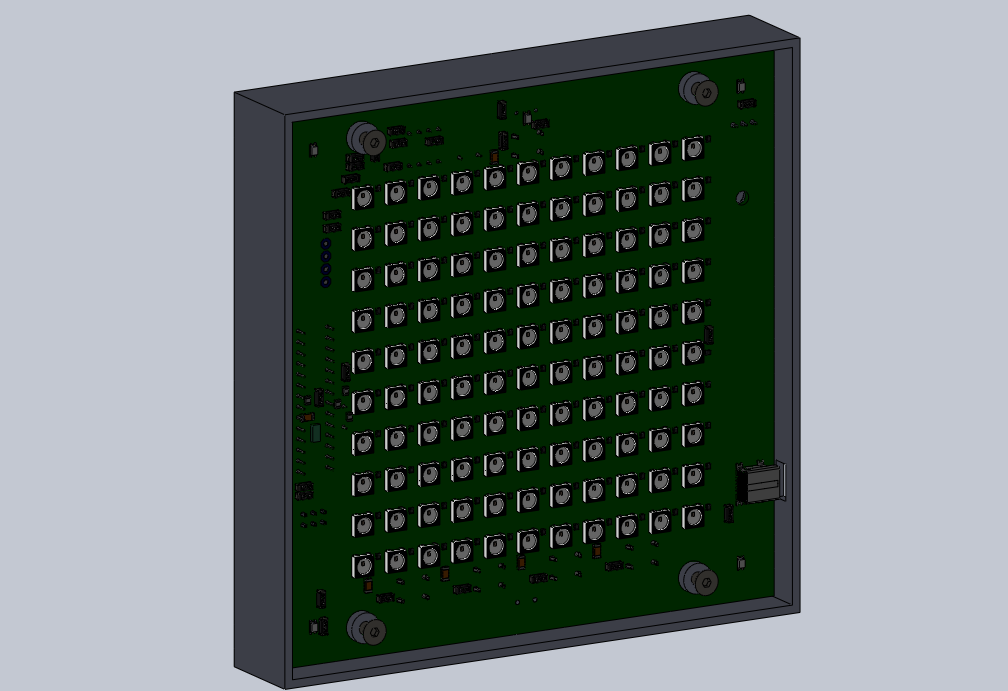
\includegraphics[width=0.45\textwidth]{Bilder/SW2}
	\caption{Das erstellte Modell mit der eingebauter Elektronik} 
	\label{fig:SW2}
\end{figure}
Für den Prototyp wurde das Gehäuse mit dem Onlinetool \glqq Boxmaker\grqq aus Akryl ausgelasert. Die Zwischenplatte, die dazu dient die einzelnen LEDs gegeneinander abzuschirmen wurde ebenfalls zuerst in SolidWorks erstellt und anschließend mit dem Lasercutter aus einer MDF Platte.
Die Dicke der Zwischenplatte ergibt sich aus dem Abstrahlwinkel der LEDs, dieser beträgt bei den WS2812B 120°. Für die Dicke der Zwischenplatte ergibt sich also mit einer Buchstabengröße von etwa 8mm: 
\begin{equation}
d = \frac{\frac{1}{2} * Buchstabendurchmesser}{tan\frac{120^\circ }{2}}= 4,62
\end{equation}
Aus diesem Grund wurde eine Dicke von 5mm für die Zwischenplatte gewählt.
Zusammengehalten wird die gesamte Uhr von vier M3 Schrauben, welche die Platine, die Zwischenplatte und das Gehäuse mit Abstandshalter fixieren, damit diese nicht verrutschen.
\begin{figure}[h]
	\centering
	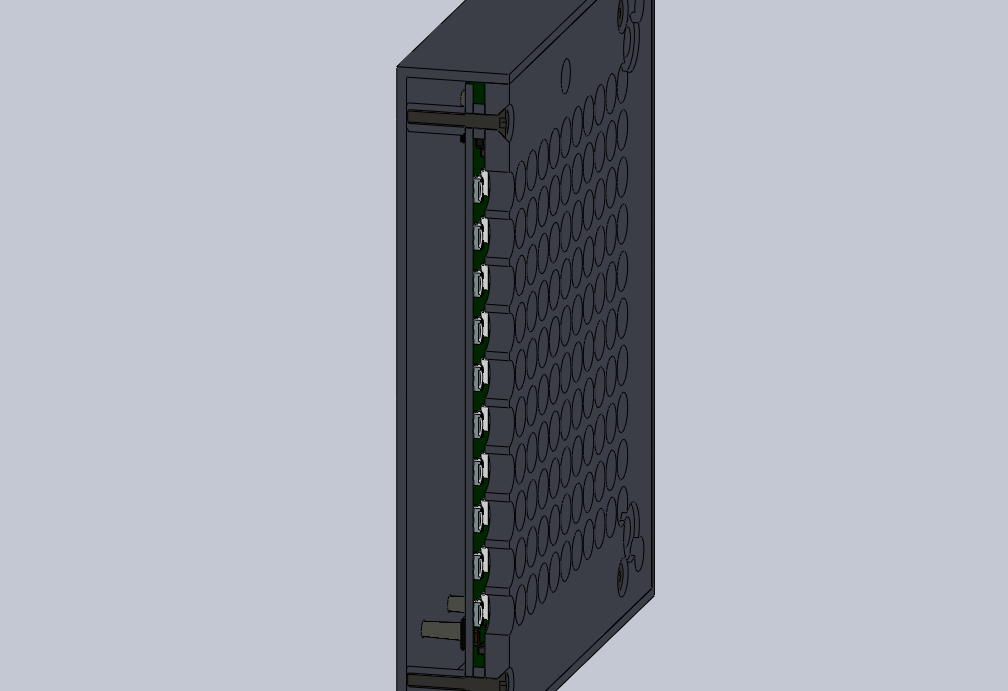
\includegraphics[width=0.45\textwidth]{Bilder/SW3}
	\caption{Schnitt durch das in SolidWorks erstellte Modell} 
	\label{fig:SW3}
\end{figure}


\subsection{Frontplatten}
Für die Frontplatte wurde die Anordnung der Buchstaben in einer Illustrator-Datei erstellt. Dabei wurden alle Buchstaben so angeordnet, dass diese exakt über das entsprechende Loch in der Zwischenplatte passen. Für die erste Anordnung der Buchstaben wurde das selbe Schema, welches auch bei der Qlocktwo und vielen weiteren Wordclocks im Internet zu finden ist, angewendet. Außerdem wurde eine Frontplatte erstellt, die es ermöglicht die Wordclock auch als Binäruhr zu verwenden. 
\begin{figure}[h]
	\centering
	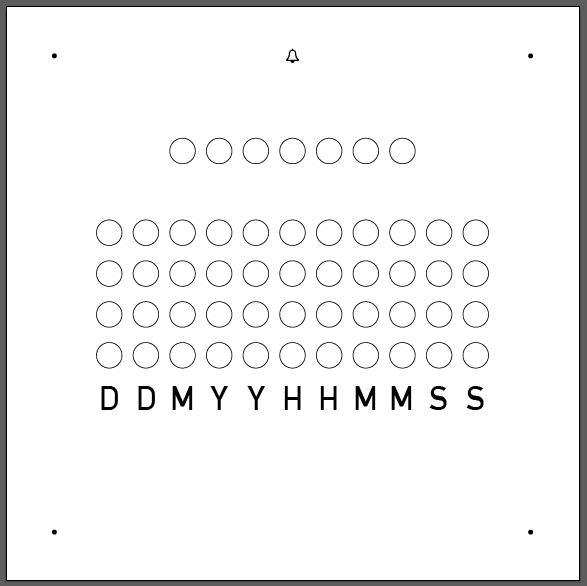
\includegraphics[width=0.45\textwidth]{Bilder/Frontplatte2}
	\caption{Eine Binäre Frontplatte für die Wordclock mit Anzeige für Wochentag (oben), Datum und Uhrzeit} 
	\label{fig:Frontplatte2}
\end{figure}
Hierfür muss nur die Software entsprechend angepasst werden. Da die Frontplatte idealerweise  nur an den Buchstaben das Licht durchlässt und dort leicht milchig sein sollte, gibt es  verschiedene Möglichkeiten zum Herstellen der Platte. Die simpelste Möglichkeit ist dabei, das Layout der Frontplatte auf mehrere Overheadfolien zu drucken und diese mit einem Blatt Papier als Diffusor gemeinsam zu laminieren. Problematisch ist hierbei allerdings die Verbindung der einzelnen Folien, da diese sich leicht lösen. Bei der binären Frontplatte wurden nur die Lichtdurchlässe aus der Holzplatte ausgeschnitten, die hierfür verwendet wurde. Diese wurden anschließend von hinten mit Papier verklebt, sodass die LEDs durch dieses diffus hindurchleuchten. Als aufwendigste Methode wurde  eine Akrylscheibe von hinten zuerst farbig und anschließend mehrfach schwarz lackiert. Aus dieser wurde das in Illustrator erstellte Frontplattenlayout dann ausgraviert. Die Schwarze Lackierung dient hierbei dazu, dass die LEDs nicht durch die farbigen Stellen der Frontplatte hindurch leuchten. Eine weitere, aber nicht erprobte Methode, wäre das Ausschneiden einer Folie mit dem im Fablab verfügbaren Folienplotter, diese wurde anschließend auf eine Milchglasscheibe geklebt. Alle Frontplatten sind mit einem Magnet an der Zwischenplatte befestigt, so wird kein Werkzeug zum Austauschen der Zwischenplatte benötigt.



\section{Software}
Die Software für den Atmega168 wurde in Eclipse entwickelt. Der wesentliche Teil der Software ist die Ansteuerung der Matrix aus 110 WS2812B LEDs. Diese funktioniert über ein spezielles Protokoll: die erste LED der Matrix bekommt einen Strom an Bits vom Mikrocontroller. Von diesem Bitstrom entfernt die erste LED die vordersten 24 Bit und gibt alle weiteren ankommenden Bits an die nächste LED weiter, die nach dem selben Prinzip verfährt. Somit erhält jede LED 24 bit, von denen jeweils 8 die Helligkeit der drei Farben Grün, Rot und Blau repräsentieren. Die 8 Bit kodieren dabei die Helligkeit der jeweiligen Farbe in 256 Stufen. Die Übertragung zu den WS2812B erfolgt durch ein unipolares Non-Return-To-Zero-Signal. Eine 1 wird dabei durch einen nur 0,2us längeren Impuls als eine 0 übertragen; Aus diesem Grund ist, die Ansteuerung sehr zeitkritisch und Interrupts sollten während des Senden an die LED-Matrix deaktiviert sein.
\begin{figure}[h]
	\centering
	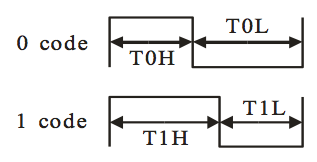
\includegraphics[width=0.45\textwidth]{Bilder/WS2812Code}
	\caption{Ausschnitt aus dem Datenblatt der WS2812B} 
	\label{fig:WS2812Code}
\end{figure}
Zur Ansteuerung wird die light\_ws2812 V2.3 von cpldcpu verwendet, die auf Github unter der GNU General Public License veröffentlicht ist. Diese Bibliothek übernimmt vom Hauptprogramm einen selbst definierten Datentyp, der für jede Farbe ein Array mit allen 110 LEDs der Matrix enthält. Den LEDs können  somit getrennte Helligkeitswerte zugewiesen werden. Um Probleme bei der Ansteuerung der letzten LED zu umgehen, wurde das Array jedoch um eines länger gewählt, als die Matrix eigentlich ist. Dies führt dazu, dass die letzte WS2812B noch immer Daten weiterreichen muss und somit die Wahrscheinlichkeit  durch einen Bitfehler eine falsche Helligkeit anzuzeigen sinkt.
Die  Verbindung zum DS1337 Bausteil erfolgt, wie bereits erwähnt über das Two-Wire-Interface und verwendet dabei die eingebaute Peripherie des AVR. Softwareseitig baut die Kommunikation auf einer Bibliothek auf, die eigentlich für den Bausteil DS1307 gedacht ist. Diese wurde von Davide Gironi  ebenfalls unter der GNU General Public License zur Verfügung gestellt. Da sich die beiden Bausteine in Ihren Registern für die Stunden, Minuten und Sekunden sowie denen für das Datum aber entsprechen, funktioniert diese Library auch um das Datum im DS1337 zu speichern und aus diesem auch zu lesen. 

\section{Ausblick}
Bisher noch nicht umgesetzt wurde die Einstellung der aktuellen Uhrzeit mit den fünf zur Verfügung stehenden Tastern. Dafür soll entweder die Möglichkeit des AVR genutzt werden einen Pin-change-Interrupt  bei einem Tastendruck zu generieren. Alternativ könnte in der Hauptschleife ständig abgefragt werden, ob die Taste gerade gedrückt wurde. In einer späteren Version der Wordclock wäre es auch noch wünschenswert, wenn die Taster  beschriften werden würden. Dies wäre auf dem Gehäuse ohne Probleme mit dem Lasercutter zu realisieren.
Da die Bibliothek für die Kommunikation mit der Realtime-Clock aktuell die Verwendung der im Baustein DS1337 verfügbaren Alarme nicht unterstützt müsste die Kommunikation noch um einige Funktionen erweitert werden, damit auch die Alarme des Bausteins genutzt werden können. Intern nutzt die Bibliothek für die Konfiguration der Uhr einige Funktionen zum Senden und Empfangen von Daten über das Two-Wire-Interface. Diese könnten sicher auch bei der weiteren Anpassung der Bibliothek an den DS1337 Baustein verwendet werden.
Weitere Features wie der Empfang der aktuellen Zeit über den Sender DCF77, also der Umbau zu einer Funkuhr wären ebenfalls leicht möglich. Dafür könnten die bereits erwähnten Durchkontaktierungen in der Platine und die beiden ungebelgten Pins des Atmega genutzt werden. Zwischen der Platine und der Rückwand des Gehäuses wäre auch noch genügend Luft vorhanden, in den ein solcher Empfänger eingebaut werden könnte. Alternativ kann hier aber auch eine Lösung gut untergebracht werden, die die Uhr zu einer batteriebetriebnen Wordclock erweitert. Der einfachste Weg dazu wäre, eine USB-Powerbank zu nutzen, da diese integriert bereits Elektrische Schaltungen zum Laden der Akkus und eine Spannungsstabilisierung auf die benötigten 5V hat.
Da die Buchstaben alle einzeln ansteuerbar sind, besteht auch die Möglichkeit die Matrix für noch weitere Anwendungen zu nutzen. Denn durch die vielen LEDs können auch Muster wie Kreise oder andere Formen auf der Matrix angezeigt werden. So kann etwa auch die Temperatur angezeigt werden oder alternativ das Datum oder der Wochentag. Dafür würden solche LEDs aktiviert, die zusammen den Umriss eines gewünschten Buchstaben oder einer Zahl bilden, der sich über die gesamte Matrix erstreckt.
\begin{figure}
	\centering
	\includegraphics[width=0.45\textwidth]{Bilder/FotoWordclock}
	\caption{Foto der fertigen Wordclock} 
	\label{fig:Foto}
\end{figure}
%----------------------------------------------------------------------------------------------Ende des eigentlichen Textes

\nocite{*}
%\begin{thebibliography}{1}
%\bibliography{literatur.bib}
%\bibliographystyle{plain}
%\bibitem{IEEEhowto:kopka}
%H.~Kopka and P.~W. Daly, \emph{A Guide to {\LaTeX}}, 3rd~ed.\hskip 1em plus
 % 0.5em minus 0.4em\relax Harlow, England: Addison-Wesley, 1999.

%\end{thebibliography}




% that's all folks
\end{document}


